\documentclass{scrartcl}

% packages
\usepackage{amsmath}
\usepackage{amssymb}
\usepackage[ngerman]{babel}
\usepackage{booktabs}
\usepackage[font=small,labelfont=bf]{caption}
\usepackage{csquotes}
\usepackage{float}
\usepackage{fontspec}
  \setmainfont[Ligatures=TeX]{Tex Gyre Pagella}
\usepackage{graphicx}
 \usepackage[pdfusetitle,unicode]{hyperref}
\usepackage{mathtools}
\usepackage{microtype}
\usepackage{siunitx}
  \sisetup{separate-uncertainty=true}
\usepackage{subcaption}
\usepackage[math-style=ISO,bold-style=ISO]{unicode-math}
  %\setmathfont{"[Tex Gyre Pagella Math.ttf]"}
\usepackage{xfrac}

% options
\setlength{\parindent}{0pt}  % no stupid indentation

% commands
\DeclarePairedDelimiter{\abs}{\lvert}{\rvert}
\DeclarePairedDelimiter{\mean}{\langle}{\rangle}
\renewcommand{\vec}[1]{\mathbf{#1}}
\renewcommand{\i}{\mathrm{i}}
\DeclareRobustCommand{\e}{\ensuremath{\mathrm{e}}}

% meta
\author{Kevin Dungs \and Kevin Heinicke}
\title{Computational Physics}
\subtitle{Übungsblatt 1}

% document
\begin{document}
\maketitle

\section*{Hausaufgabe 3: Berechnung von $\mathbf{\pi}$}
Siehe \texttt{pi.cc}. \\

Insgesamt ist die Methode zur Annäherung von $\pi$ nicht zu empfehlen. Sie konvergiert sehr langsam und auch die Berechnung ist auf Grund der Verwendung von Zufallszahlen langsam. Eine bessere Methode wäre zum Beispiel ein Algorithmus mit quadratischer Konvergenz basierend auf der AGM-Methode.

\section*{Hausaufgabe 4: Random-Walk mit Selbstüberschneidung}
Seien $i$ alle möglichen Wege eines Random-Walks gegebener Länge $N$ und $d$ die Dimension, sowie $\vec{e}$ die Einheitsvektoren, folgt für die mittlere Clustergröße eines Random-Walks nach einem Schritt $R_1$:
    \begin{eqnarray*}
        R_1^2 \quad = \quad \langle \vec{r}^2(1) \rangle & = & \sum_i p_i \sum_{k=1}^{2d} \frac{1}{2d}\left(\vec{0} + \vec{e}_k \right)^2 \\
        & = & 1 \\
    \end{eqnarray*}
Der Induktionsschritt liefert die gewünschte Propotionalität:
    \begin{eqnarray*}
        R_{N+1}^2 \quad = \quad \langle \vec{r}^2(N+1) \rangle & = & \sum_i p_i \sum_{k=1}^{2d} \left( \vec{r}_i + \vec{e}_k \right)^2 \\
                                                               & = & \sum_i \frac{p_i}{2d} \left\{ \left( \vec{r}_i + \vec{e}_{x_1} \right)^2 + \left( \vec{r}_i - \vec{e}_{x_1} \right)^2 \right. \\ 
                                                               & & \left. + \dots + \left( \vec{r}_i + \vec{e}_{x_d} \right)^2 + \left( \vec{r}_i - \vec{e}_{x_d} \right)^2 \right\} \\
                                                               & = & \sum_i \left( p_i \vec{r}_i^2 + p_i \right) \\
                                                               & = & \langle \vec{r}^2(N) \rangle + 1 \\
                                                               & \propto & N + 1 \\
        \Rightarrow \quad R_N^2 \quad \propto & N & \propto \quad t
    \end{eqnarray*}


\section*{Hausaufgabe 5: Random-Walk ohne Selbstüberschneidung}
Siehe \texttt{saw.cc}. \\

In \autoref{fig:exponents} sind exemplarisch zwei Plots mit verschiedenen Exponenten abgebildet. Wie auch insbesondere aus den p-Werten der linearen Ausgleichsrechnung \eqref{eq:pvalues} hervorgeht, lässt sich der Exponent anhand der Daten nicht klar bestimmen.

\begin{equation} \label{eq:pvalues}
    p_{4/3} = \num{1.531e-08} \quad\quad p_1 = \num{2.654e-11}
\end{equation}

\begin{figure}[H]
  \centering
  \begin{subfigure}{.48\textwidth}
    \centering
    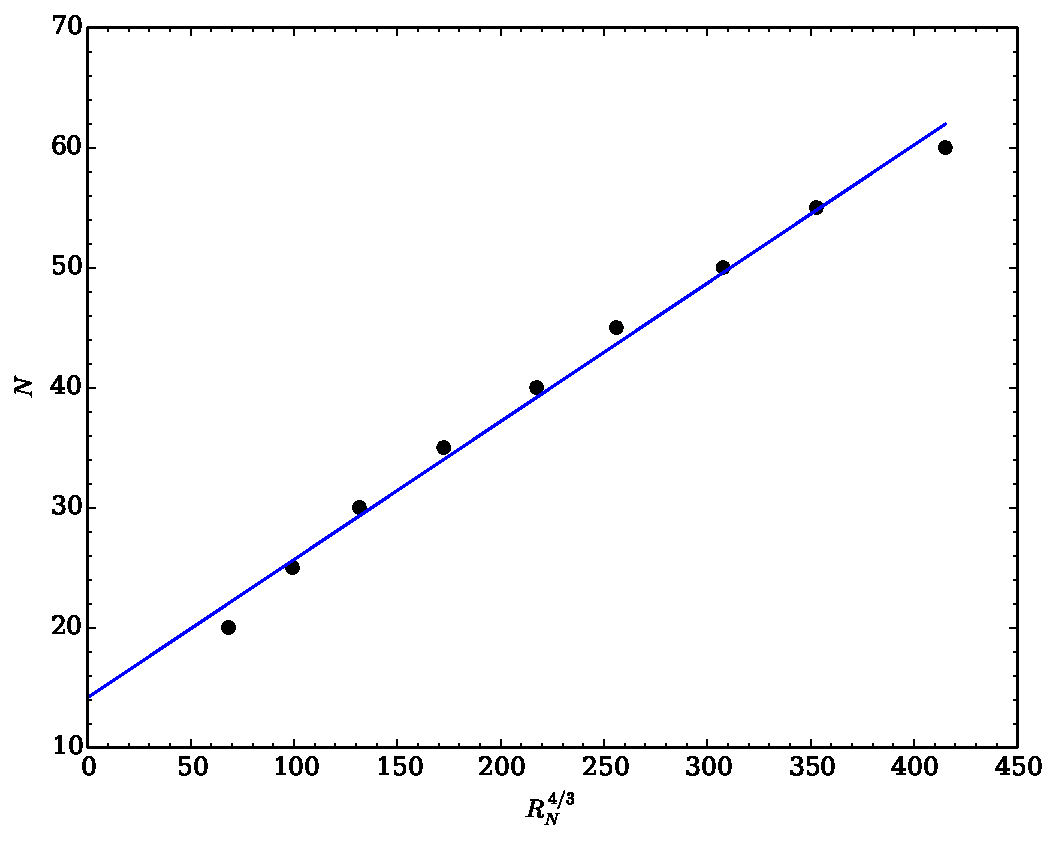
\includegraphics[width=\textwidth]{plots/saw_N_RN43.pdf}
  \end{subfigure}
  \begin{subfigure}{.48\textwidth}
    \centering
    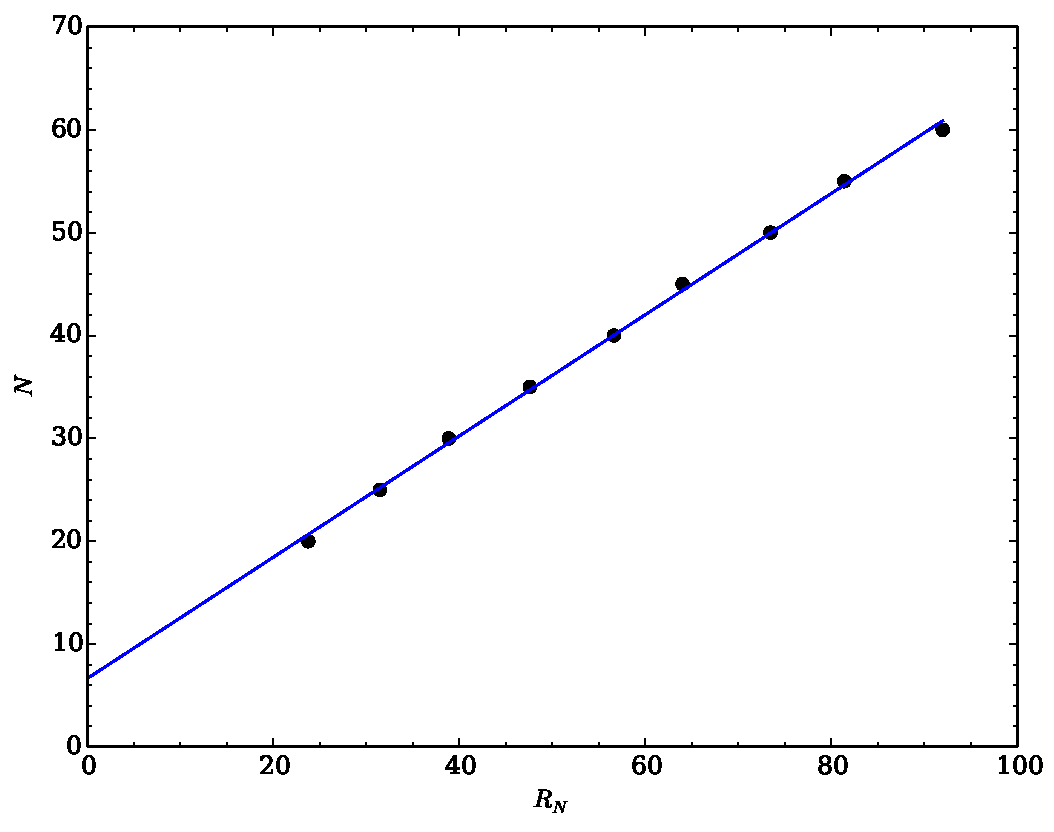
\includegraphics[width=\textwidth]{plots/saw_N_RN.pdf}
  \end{subfigure}
  \caption{Exemplarische Plots zur Bestimmung des Exponenten.}
  \label{fig:exponents}
\end{figure}


\end{document}
